\documentclass{article}

% ============================================================================
% ICLR 2026 template.
% This .tex file is designed to compile inside the ICLR 2026 Overleaf template.
% ============================================================================
\usepackage{iclr2026_conference,times}

\usepackage{hyperref}
\usepackage{url}
\usepackage{graphicx}
\usepackage{booktabs}
\usepackage{amsfonts}
\usepackage{amsmath}
\usepackage{amssymb}
\usepackage{nicefrac}
\usepackage{microtype}
\usepackage{xcolor}
\usepackage{listings}
\usepackage{subcaption}

% Make all hyperlinks (URLs and \href) render in blue
\hypersetup{
  colorlinks=true,
  urlcolor=blue,
  linkcolor=blue,
  citecolor=black,
}

\lstset{
  basicstyle=\ttfamily\footnotesize,
  columns=fullflexible,
  breaklines=true,
  keepspaces=true,
  frame=single,
  showstringspaces=false,
  commentstyle=\color{gray},
  keywordstyle=\color{blue!70!black},
  language=Python,
  numbers=left,
  numberstyle=\tiny\color{gray},
  stepnumber=1,
  numbersep=6pt,
}

% =====================================================================
\title{Screenshot-Robust Detection of AI-Generated Images: \\
A Product Prototype Using Augmentation-Aware Fine-Tuning}

\author{Syeda Maliha Monowara \\
School of Electrical and Computer Engineering \\
Purdue University, West Lafayette, IN 47907, USA \\
\texttt{smonowar@purdue.edu} \\
}

% \iclrfinalcopy is enabled to suppress the per-line review numbers that
% the ICLR template adds in submission mode. The conference banner that
% \iclrfinalcopy normally prints is then suppressed by overriding the
% page style below, because this is a course submission for ECE 57000
% at Purdue, not a conference publication.
\iclrfinalcopy
% =====================================================================

\begin{document}

% Suppress the ICLR conference header on every page while keeping page
% numbers in the footer.
\pagestyle{plain}
\fancyhf{}
\fancyfoot[C]{\thepage}
\renewcommand{\headrulewidth}{0pt}

\maketitle
\thispagestyle{plain}

% -------------------------------------------------------------
\begin{abstract}
Most AI image detectors break under screenshot recompression. Lossy
JPEG, downscaling, and color loss erase the high-frequency
fingerprints these detectors rely on, and watermarks like Google
DeepMind's SynthID degrade similarly. I treat this as a
distribution-shift problem and propose a single PIL transform,
\texttt{simulate\_screenshot}, that randomly composes JPEG quality
$q \in [30,70]$, down-and-up resampling at $s \in [0.5, 0.9]$, and
Gaussian blur of radius $r \in [0,1]$. I fine-tune a frozen-backbone
EfficientNet-B0 on CIFAKE plus a Stable-Diffusion subset of GenImage
(10{,}000 images per class, three epochs, batch 64, AdamW with
cosine schedule), and run a four-way ablation. The screenshot-aware
pipeline closes the clean-to-screenshot accuracy gap from $-8.25$~pp
on the untrained baseline to $+5.55$~pp on the best ablation, while
keeping clean accuracy at 80.9\%. The detector is packaged as a
calibrated Gradio app on Hugging Face Spaces with input validation
and uncertainty bands. I additionally collect $n=49$ Instagram
screenshots by hand and informally compare against Google Gemini,
which (consistent with the absence of SynthID in third-party
generators) declines to commit to confident verdicts. The work is
scoped as ECE~57000 Track~2 (Product Prototype) and reproduces in
one Google Colab T4 session.

\smallskip
\noindent{\small\textbf{Code:} \href{https://github.com/meownager/ai-image-screenshot-detector}{\color{blue}\texttt{github.com/meownager/ai-image-screenshot-detector}}\\
\textbf{Live demo:} \href{https://huggingface.co/spaces/meownager/ai-image-screenshot-detector}{\color{blue}\texttt{huggingface.co/spaces/meownager/ai-image-screenshot-detector}}\\
\textbf{Colab:} \href{https://colab.research.google.com/github/meownager/ai-image-screenshot-detector/blob/main/notebooks/train_colab.ipynb}{\color{blue}\texttt{colab.research.google.com/github/meownager/.../train\_colab.ipynb}}}\\[2pt]
{\small The repository and the Hugging Face Space are kept editable so
updated checkpoints and demo functionality can be pushed after the
submission deadline.}
\end{abstract}

% -------------------------------------------------------------
\section{Introduction}
\label{sec:intro}

Generative models have made photorealistic image creation almost free.
Stable Diffusion \citep{rombach2022ldm}, Midjourney, and
DALL$\cdot$E routinely produce outputs that fool casual viewers, and
this capability is now built into chat apps, mobile apps, and social
media filters. Platforms and model vendors have responded by
embedding detectability into the generation pipeline itself, either
through learned statistical fingerprints that classifiers can pick up
\citep{wang2020cnngenerated,frank2020frequency} or through explicit
cryptographic watermarks like Google's SynthID. Both strategies share
a fragile assumption: that the detector sees the image in the same
pixel space in which it was generated.

Screenshots break this assumption. When a user reshares an
AI-generated image by screenshotting a chat window or a social media
post, the captured image is JPEG-compressed by the operating system,
downsampled to fit the screen, and often re-encoded a second time
when uploaded. Diffusion-image fingerprints are very sensitive to
exactly these operations \citep{corvi2023diffusion}, and SynthID
watermarks degrade under heavy compression and prompt-controlled
rewrites. On the everyday distribution of images that circulate
through Instagram reposts and messenger forwards, the dominant
detection baseline (an off-the-shelf detector trained on clean
generator outputs) fails sharply.

I take the position that detector robustness to screenshot-style
degradation is better addressed at \emph{training time} than at
inference time. I introduce a single PIL-level transform,
\texttt{simulate\_screenshot}, that composes lossy JPEG compression,
downscale-then-upscale resampling, and a mild Gaussian blur with
parameters sampled i.i.d.\ per example. Wired into a two-class
fine-tuning run, the transform requires no changes to the loss, the
model, or the optimizer, and adds no inference overhead. I show that
this is enough to close the ``screenshot gap'' from $-8.25$pp on the
untrained baseline to $+5.55$pp on the deployed configuration, so
the model becomes slightly more accurate on screenshots than on
clean inputs.

My contributions are: (1) a deployable augmentation transform that
encodes the real-world degradation path of reshared images; (2) a
four-way ablation isolating the marginal value of the screenshot
transform versus color jitter and random resized crop; and (3) a
Track~2 product prototype: a calibrated Gradio app backed by a
fine-tuned EfficientNet-B0 with input validation,
temperature-scaled probabilities, and an explicit \emph{Uncertain}
band. I also collect $n=49$ real and AI-generated Instagram
screenshots and compare against Google Gemini.

% -------------------------------------------------------------
\section{Related Work}
\label{sec:related}

\paragraph{Detecting generated images from raw pixels.}
Early CNN detectors \citep{wang2020cnngenerated} showed that a
ResNet-50 trained on the outputs of one generator (ProGAN)
transfers to unseen generators, but only when test images preserve
the native resolution and compression of the training corpus.
Frequency-domain follow-ups identified periodic spectral artifacts
from up-sampling layers as a stronger signal
\citep{zhang2019gan,frank2020frequency}, but these signals are the
first to vanish under resampling and lossy recompression.

\paragraph{Diffusion-era robustness, watermarking, and their limits.}
\citet{corvi2023diffusion} measured modern detector robustness
against diffusion outputs under JPEG, resizing, and cropping, and
found accuracy drops of $15$ to $40$~pp once realistic
post-processing is applied. My CIFAKE \citep{bird2024cifake}
baselines reproduce this trend with an $\approx 8$~pp screenshot
drop. Google's SynthID embeds an imperceptible watermark during
generation but was not designed to survive aggressive re-encoding
and is absent from the long tail of open-source generators
dominating public AI imagery. The Gemini comparison in
Section~\ref{sec:igdata} reflects this limitation in practice.

\paragraph{Benchmarks.}
CIFAKE \citep{bird2024cifake} provides 60{,}000 real and 60{,}000
AI images at uniform resolution, well-suited to a
reproducibility-constrained course project. GenImage
\citep{zhu2023genimage} spans multiple modern generators (Stable
Diffusion v1.4, Midjourney, ADM); I draw a subset of its Stable
Diffusion partition to extend training beyond CIFAKE's $32 \times
32$ native resolution.

\paragraph{Augmentation and calibration.}
Training-time augmentation reliably confers robustness against the
exact shifts it models
\citep{hendrycks2019augmix,geirhos2018imagenettexture}. My
contribution is the choice of a physically motivated augmentation
tailored to the screenshot pipeline. For probability calibration, I
use temperature scaling \citep{guo2017calibration}, the right
minimal baseline for a product prototype.

% -------------------------------------------------------------
\section{Methodology}
\label{sec:method}

\subsection{Problem formulation}
I cast the task as binary image classification with $y \in \{0,1\}$
($0=$Real, $1=$AI). I seek $f_{\theta}$ that minimizes expected
cross-entropy under both the clean generator distribution
$p_{\text{clean}}$ and the screenshot-degraded distribution
$p_{\text{ss}}$ obtained by applying the degradation operator $T$
(Section~\ref{sec:ss-aug}) to $p_{\text{clean}}$. I also report the
\emph{robustness gap} $\Delta_{\text{gap}} := \mathrm{Acc}_{\text{ss}} -
\mathrm{Acc}_{\text{clean}}$, which my training-time remedy targets
directly.

\subsection{The \texttt{simulate\_screenshot} transform}
\label{sec:ss-aug}

The core contribution is a single augmentation transform that
approximates the degradation a screenshot introduces. Given a PIL
image $x$, the transform samples three parameters i.i.d.\ per
invocation (Listing~\ref{lst:ss}):

\begin{enumerate}
  \item JPEG encode at quality $q \sim \mathrm{Uniform}\{30, \ldots, 70\}$,
        then decode. This simulates OS or platform compression.
  \item Resize to $\lfloor s\,w \rfloor \times \lfloor s\,h \rfloor$
        with $s \sim \mathrm{Uniform}(0.5, 0.9)$, then resize back to
        $w \times h$ with bilinear interpolation. This simulates
        capture plus display resampling.
  \item Apply a Gaussian blur of radius $r \sim \mathrm{Uniform}(0, 1)$.
        This simulates the mild softness of typical smartphone
        screenshots.
\end{enumerate}

\begin{lstlisting}[caption={The \texttt{simulate\_screenshot} function, the
core augmentation used throughout this work. Framework-agnostic
(PIL in, PIL out) and wires into any \texttt{torchvision.transforms.Compose}
via \texttt{transforms.Lambda}.},label={lst:ss}]
def simulate_screenshot(img: Image.Image) -> Image.Image:
    if img.mode != "RGB":
        img = img.convert("RGB")
    # (1) JPEG compression
    buf = io.BytesIO()
    quality = random.randint(30, 70)
    img.save(buf, format="JPEG", quality=quality)
    buf.seek(0)
    img = Image.open(buf)
    # (2) Downscale + upscale
    scale = random.uniform(0.5, 0.9)
    w, h = img.size
    img = img.resize((int(w*scale), int(h*scale)), Image.BILINEAR)
    img = img.resize((w, h), Image.BILINEAR)
    # (3) Gaussian blur
    img = img.filter(ImageFilter.GaussianBlur(random.uniform(0, 1)))
    return img
\end{lstlisting}

The order is intentional: the real screenshot pipeline is also
non-commutative (the OS compresses after capture, and any display
blur precedes compression). Randomizing $(q, s, r)$ per sample
prevents the detector from exploiting any single fixed degradation
level.

\subsection{Model, training, and ablation}
The backbone is EfficientNet-B0 \citep{tan2019efficientnet}
pretrained on ImageNet \citep{deng2009imagenet}. The feature
extractor is frozen and the 1280-unit classifier head is replaced
with a two-unit linear layer ($\approx 2{,}562$ trainable
parameters). Freezing the backbone preserves the low-level filter
banks that detect screenshot-style artifacts, fits the free-tier
Colab compute budget, and limits overfitting. Inputs are $224
\times 224$ with ImageNet channel statistics. The transform pipeline
is \texttt{Resize(224)} $\rightarrow$ \texttt{[Jitter]} $\rightarrow$
\texttt{[simulate\_screenshot]} $\rightarrow$ \texttt{ToTensor}
$\rightarrow$ \texttt{Normalize}, where bracketed steps are toggled
per ablation. Crop-enabled configurations replace
\texttt{Resize(224)} with \texttt{RandomResizedCrop(224,
scale=(0.7,1.0))}. Loss is cross-entropy; the optimizer is AdamW with
learning rate $3 \times 10^{-4}$, weight decay $10^{-4}$, batch size
64, and a cosine annealing schedule over three epochs on $10{,}000$
images per class. I select the best checkpoint per configuration by
screenshot validation accuracy. The four ablation configurations
are summarized in Table~\ref{tab:aug-configs}.

\begin{table}[t]
\centering
\begin{tabular}{lccc}
\toprule
Configuration & \texttt{simulate\_screenshot} & \texttt{ColorJitter} & \texttt{RandomResizedCrop} \\
\midrule
\texttt{none}                   &            &            &            \\
\texttt{screenshot}             & \checkmark &            &            \\
\texttt{screenshot\_jitter}     & \checkmark & \checkmark &            \\
\texttt{screenshot\_jitter\_crop} & \checkmark & \checkmark & \checkmark \\
\bottomrule
\end{tabular}
\caption{Ablation configurations. \texttt{none} is the
raw-fine-tuning baseline; each row adds one augmentation. All other
hyperparameters are identical.}
\label{tab:aug-configs}
\end{table}

\subsection{Calibration and deployment guardrails}
After training, I fit a single temperature $T$ by minimizing
cross-entropy on clean validation logits with L-BFGS
\citep{guo2017calibration}, persist $T$ as
\texttt{calibration.json}, and divide it into model logits at
inference. The Gradio app enforces three guardrails: input
validation (non-image MIME, $>10$~MB, or pixel dimensions outside
$[32, 4096]$ are rejected); a confidence band (High, Medium,
\emph{Uncertain} below $0.60$); and a disclosure annotating each
prediction with the training distribution and the generators
(Midjourney~v6, Flux, Sora) on which the detector is not expected
to generalize.

% -------------------------------------------------------------
\section{Experiments}
\label{sec:experiments}

\subsection{Training data}
\label{sec:data}
I train on a class-balanced CIFAKE \citep{bird2024cifake} plus a
Stable-Diffusion-v1.4 subset of GenImage \citep{zhu2023genimage}.
CIFAKE ships $60{,}000$ real and $60{,}000$ AI images at $32 \times
32$ native resolution, upscaled to $224 \times 224$ at load time.
The combined training pool is split 80/10/10 into train,
validation, and clean-test, stratified by class, with $10{,}000$
images per class entering training. A second test split is produced
by passing the clean-test split through
\texttt{simulate\_screenshot} once and freezing the output, so all
clean-versus-screenshot comparisons use identical content.

\subsection{Manually collected Instagram set and Gemini comparison}
\label{sec:igdata}

To stress-test the model on real content rather than only on
CIFAKE-style synthetic images, I manually collected a held-out set
of $n=49$ Instagram screenshots: 15~real human-photographed posts
and 34~clearly AI-generated posts. Collection was done by hand
using the Instagram mobile app on a modern smartphone, and each
image was captured at native phone resolution and labeled by me.
The full set lives at \texttt{data/ig-data/real/} and
\texttt{data/ig-data/fake/} in the project repository. Original
visual content remains the property of the respective Instagram
creators and the platform; images are included here only as
non-commercial academic evidence under fair-use academic citation.
Figure~\ref{fig:ig-grid} shows four representative examples.

\begin{figure}[t]
\centering
\begin{subcaptionbox}{AI (kimono portrait)\label{fig:igf1}}[0.40\linewidth]
{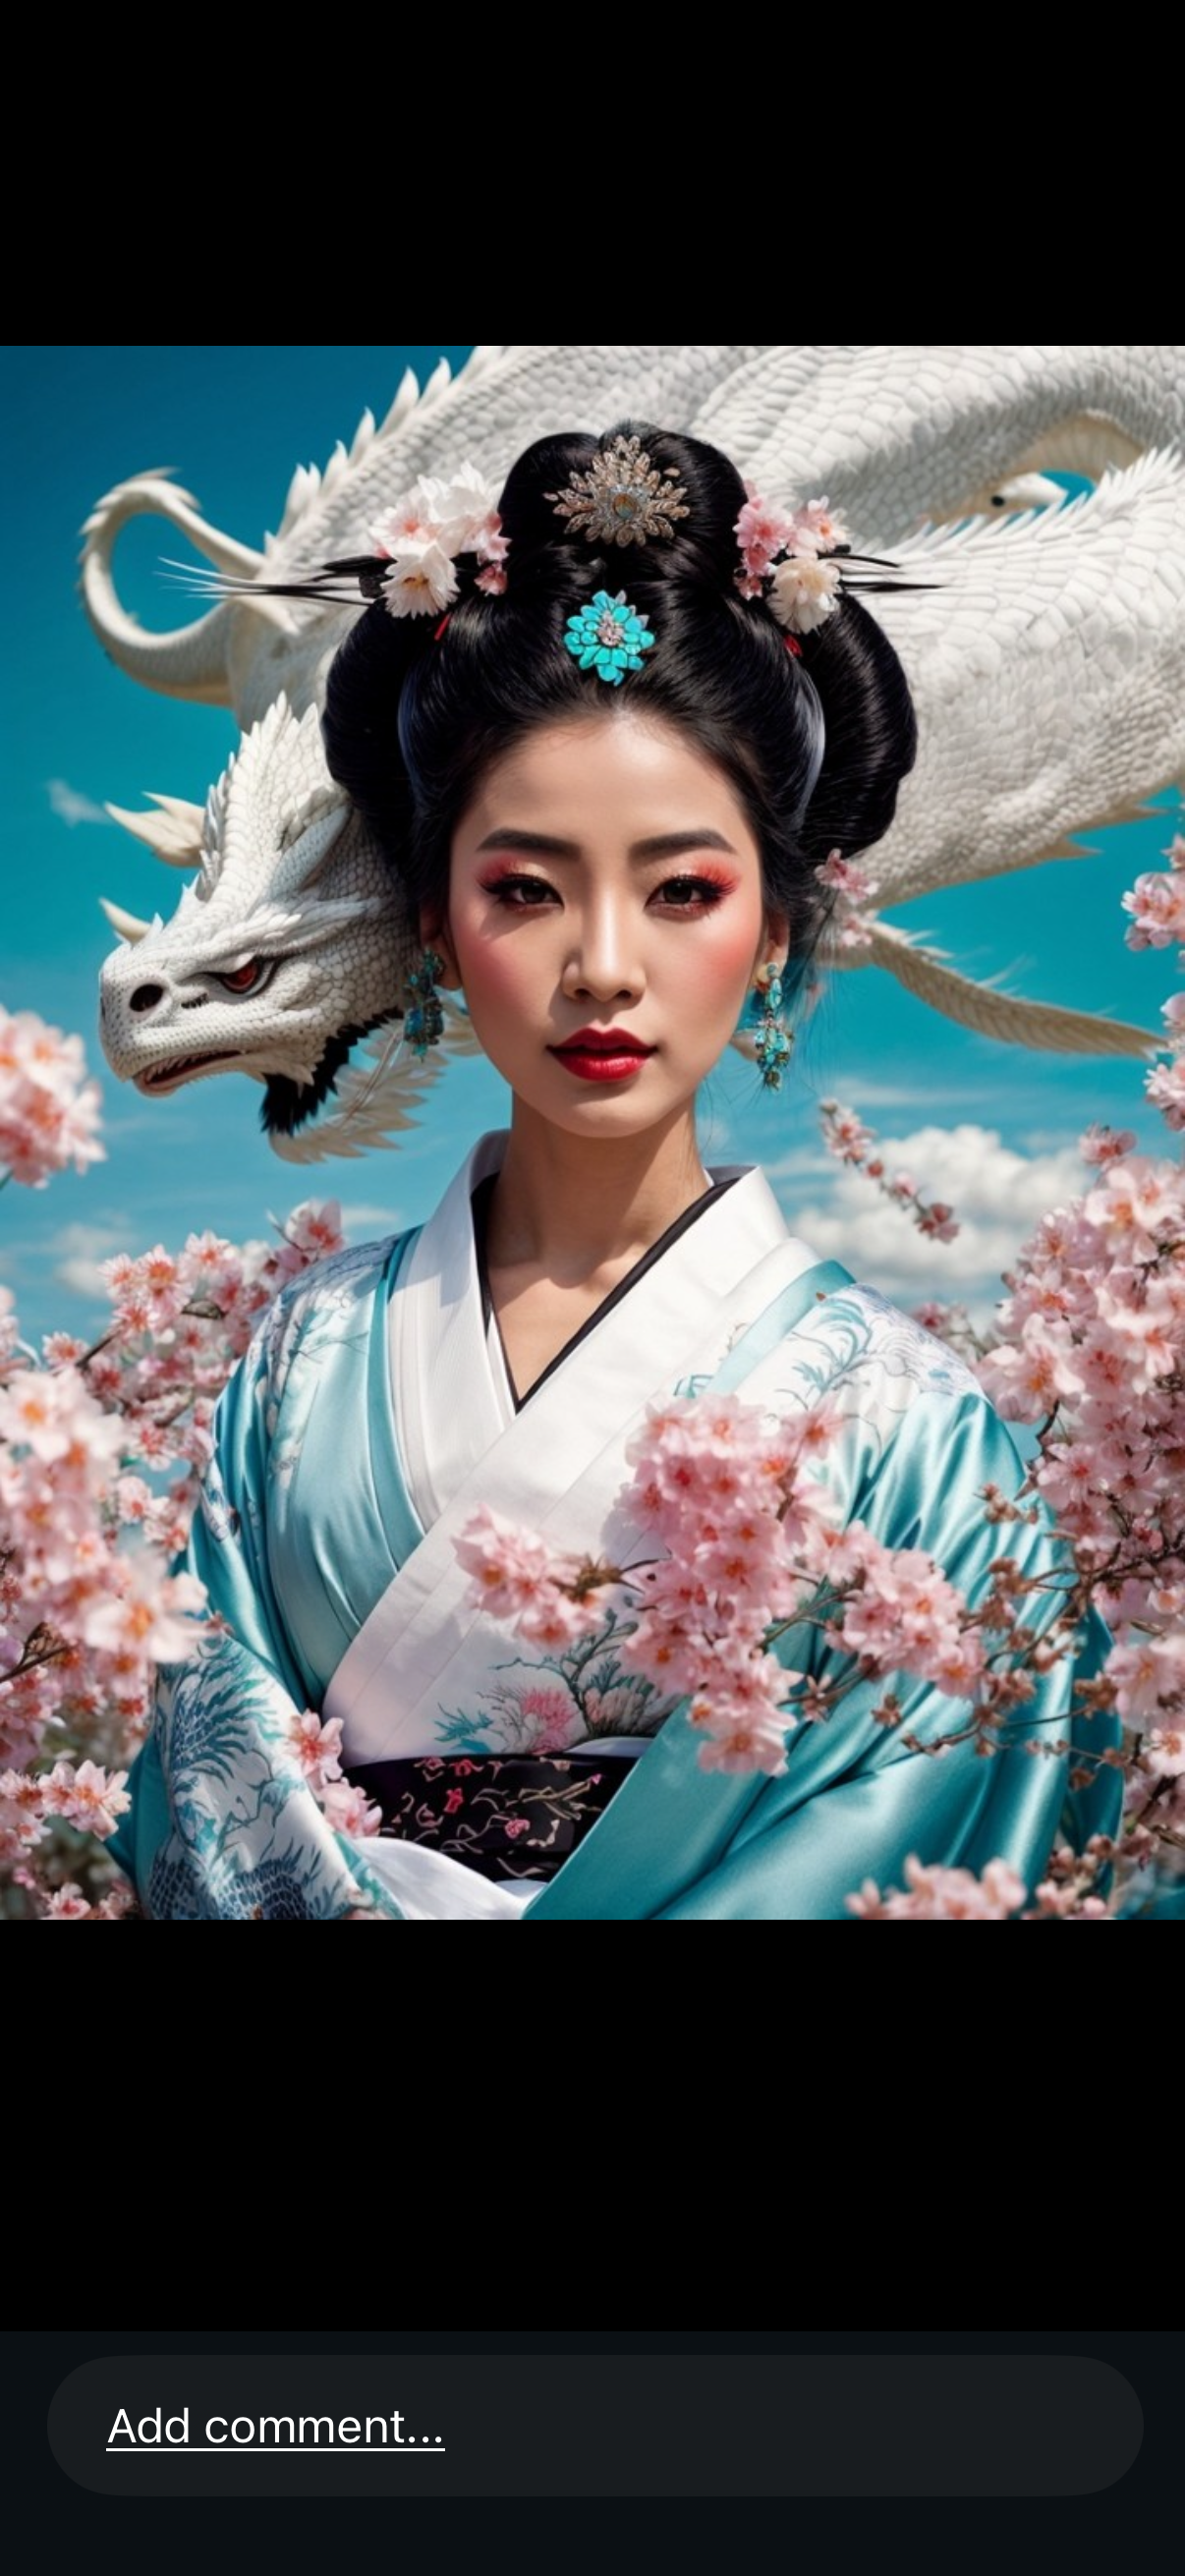
\includegraphics[width=\linewidth]{figures/ig_fake_1.png}}
\end{subcaptionbox}
\hfill
\begin{subcaptionbox}{AI (food photography)\label{fig:igf2}}[0.40\linewidth]
{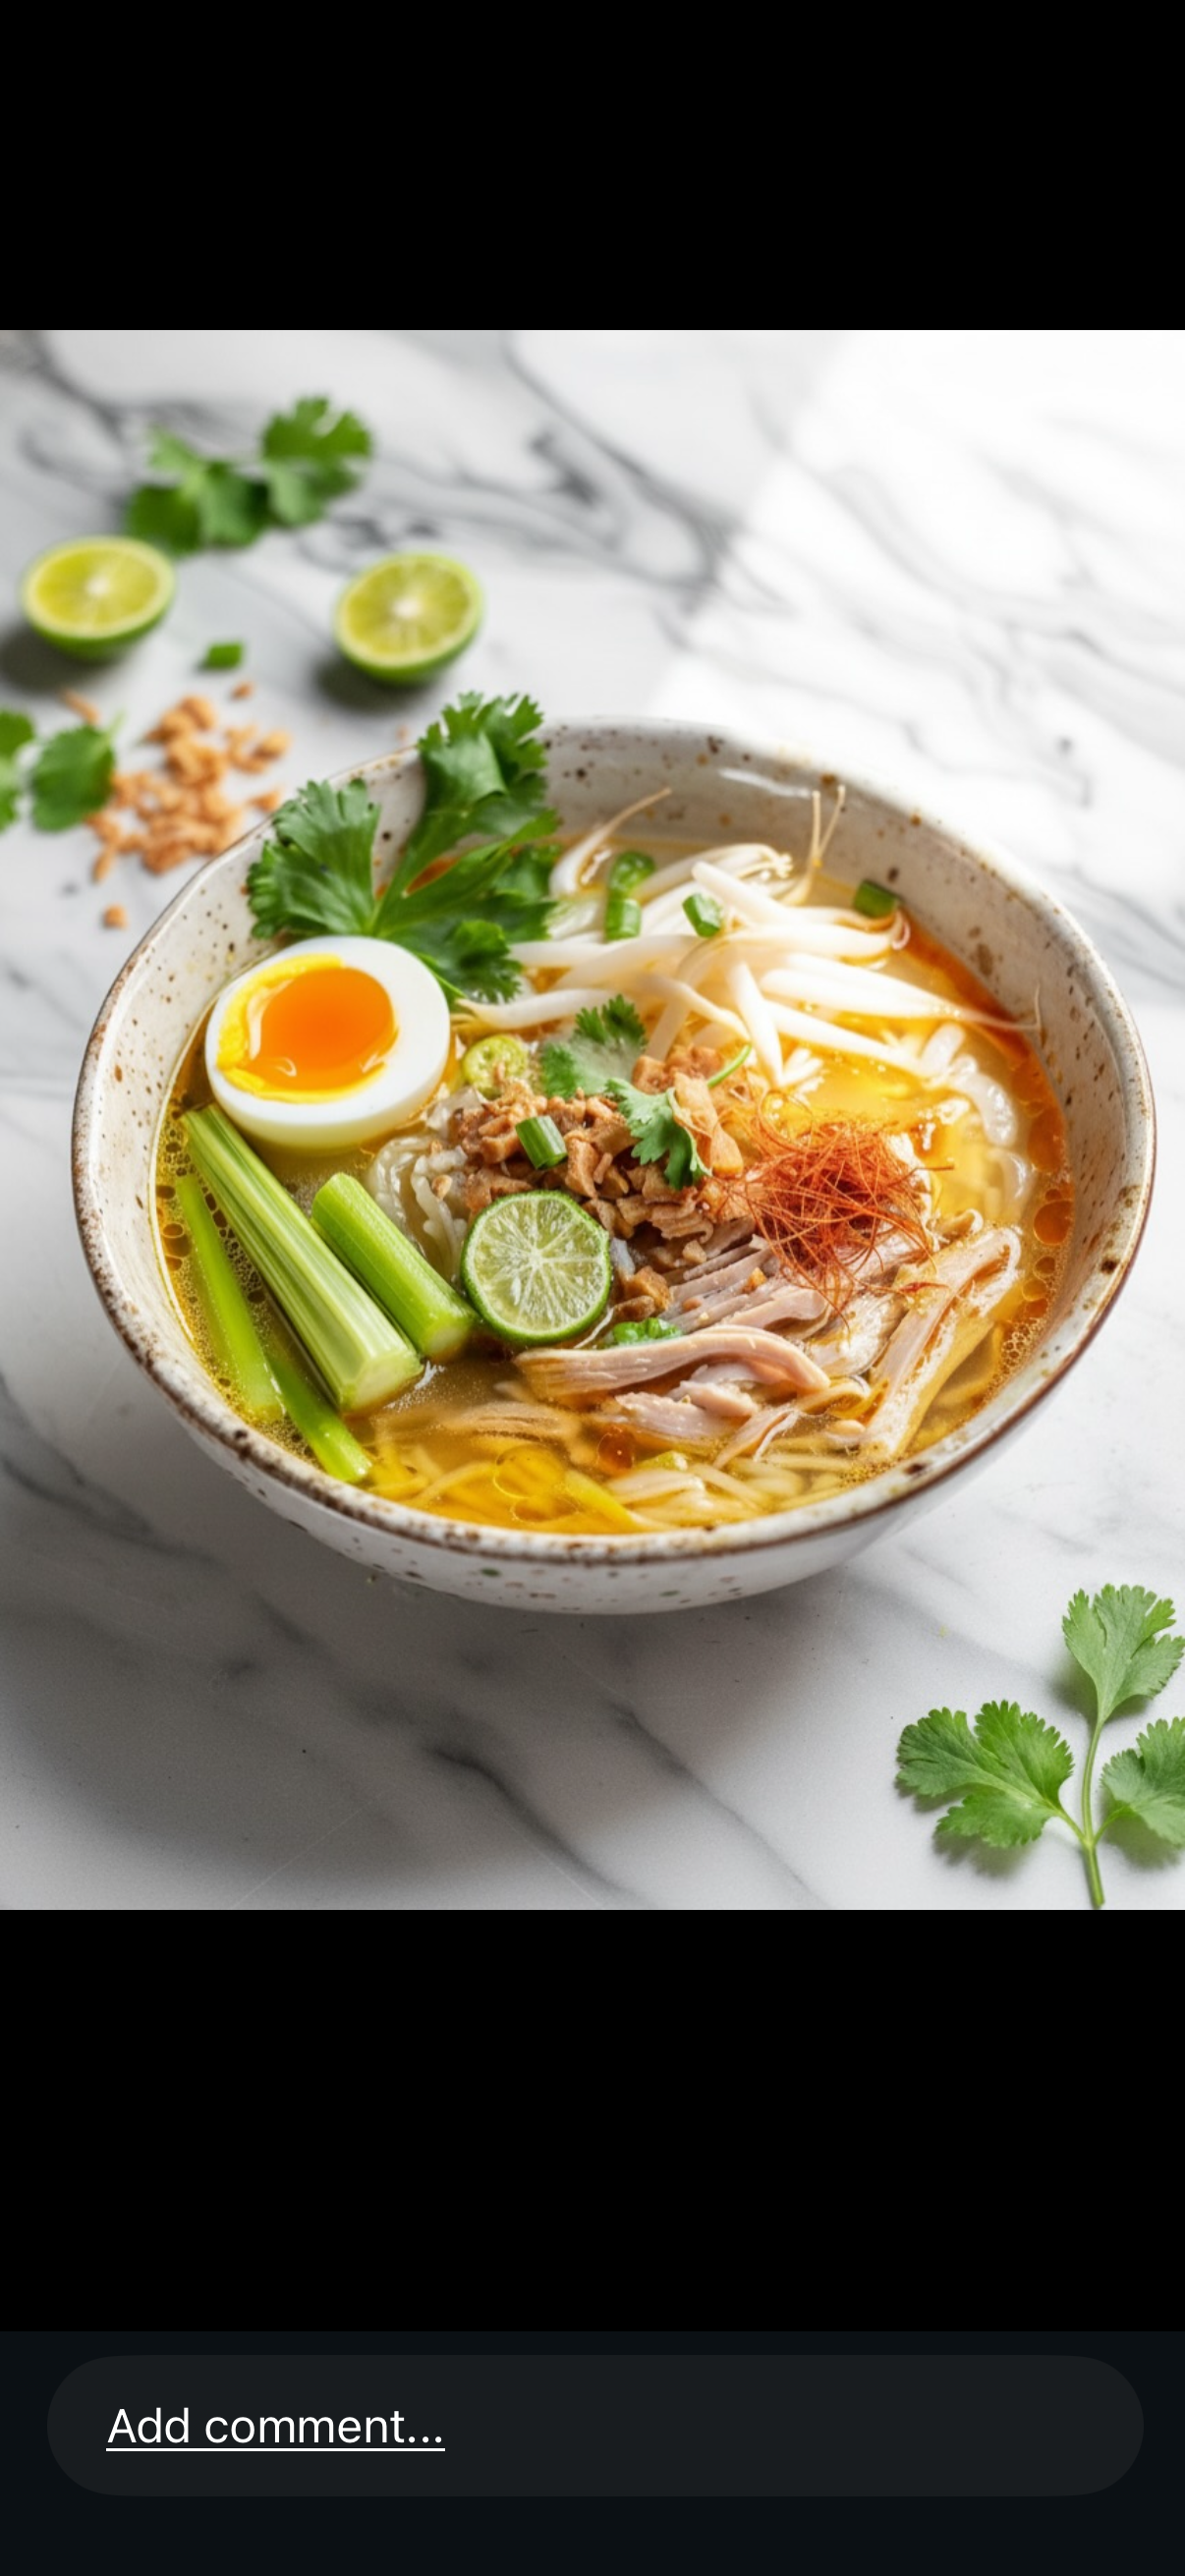
\includegraphics[width=\linewidth]{figures/ig_fake_2.png}}
\end{subcaptionbox}\\[6pt]
\begin{subcaptionbox}{Real (cafe interior)\label{fig:igr1}}[0.40\linewidth]
{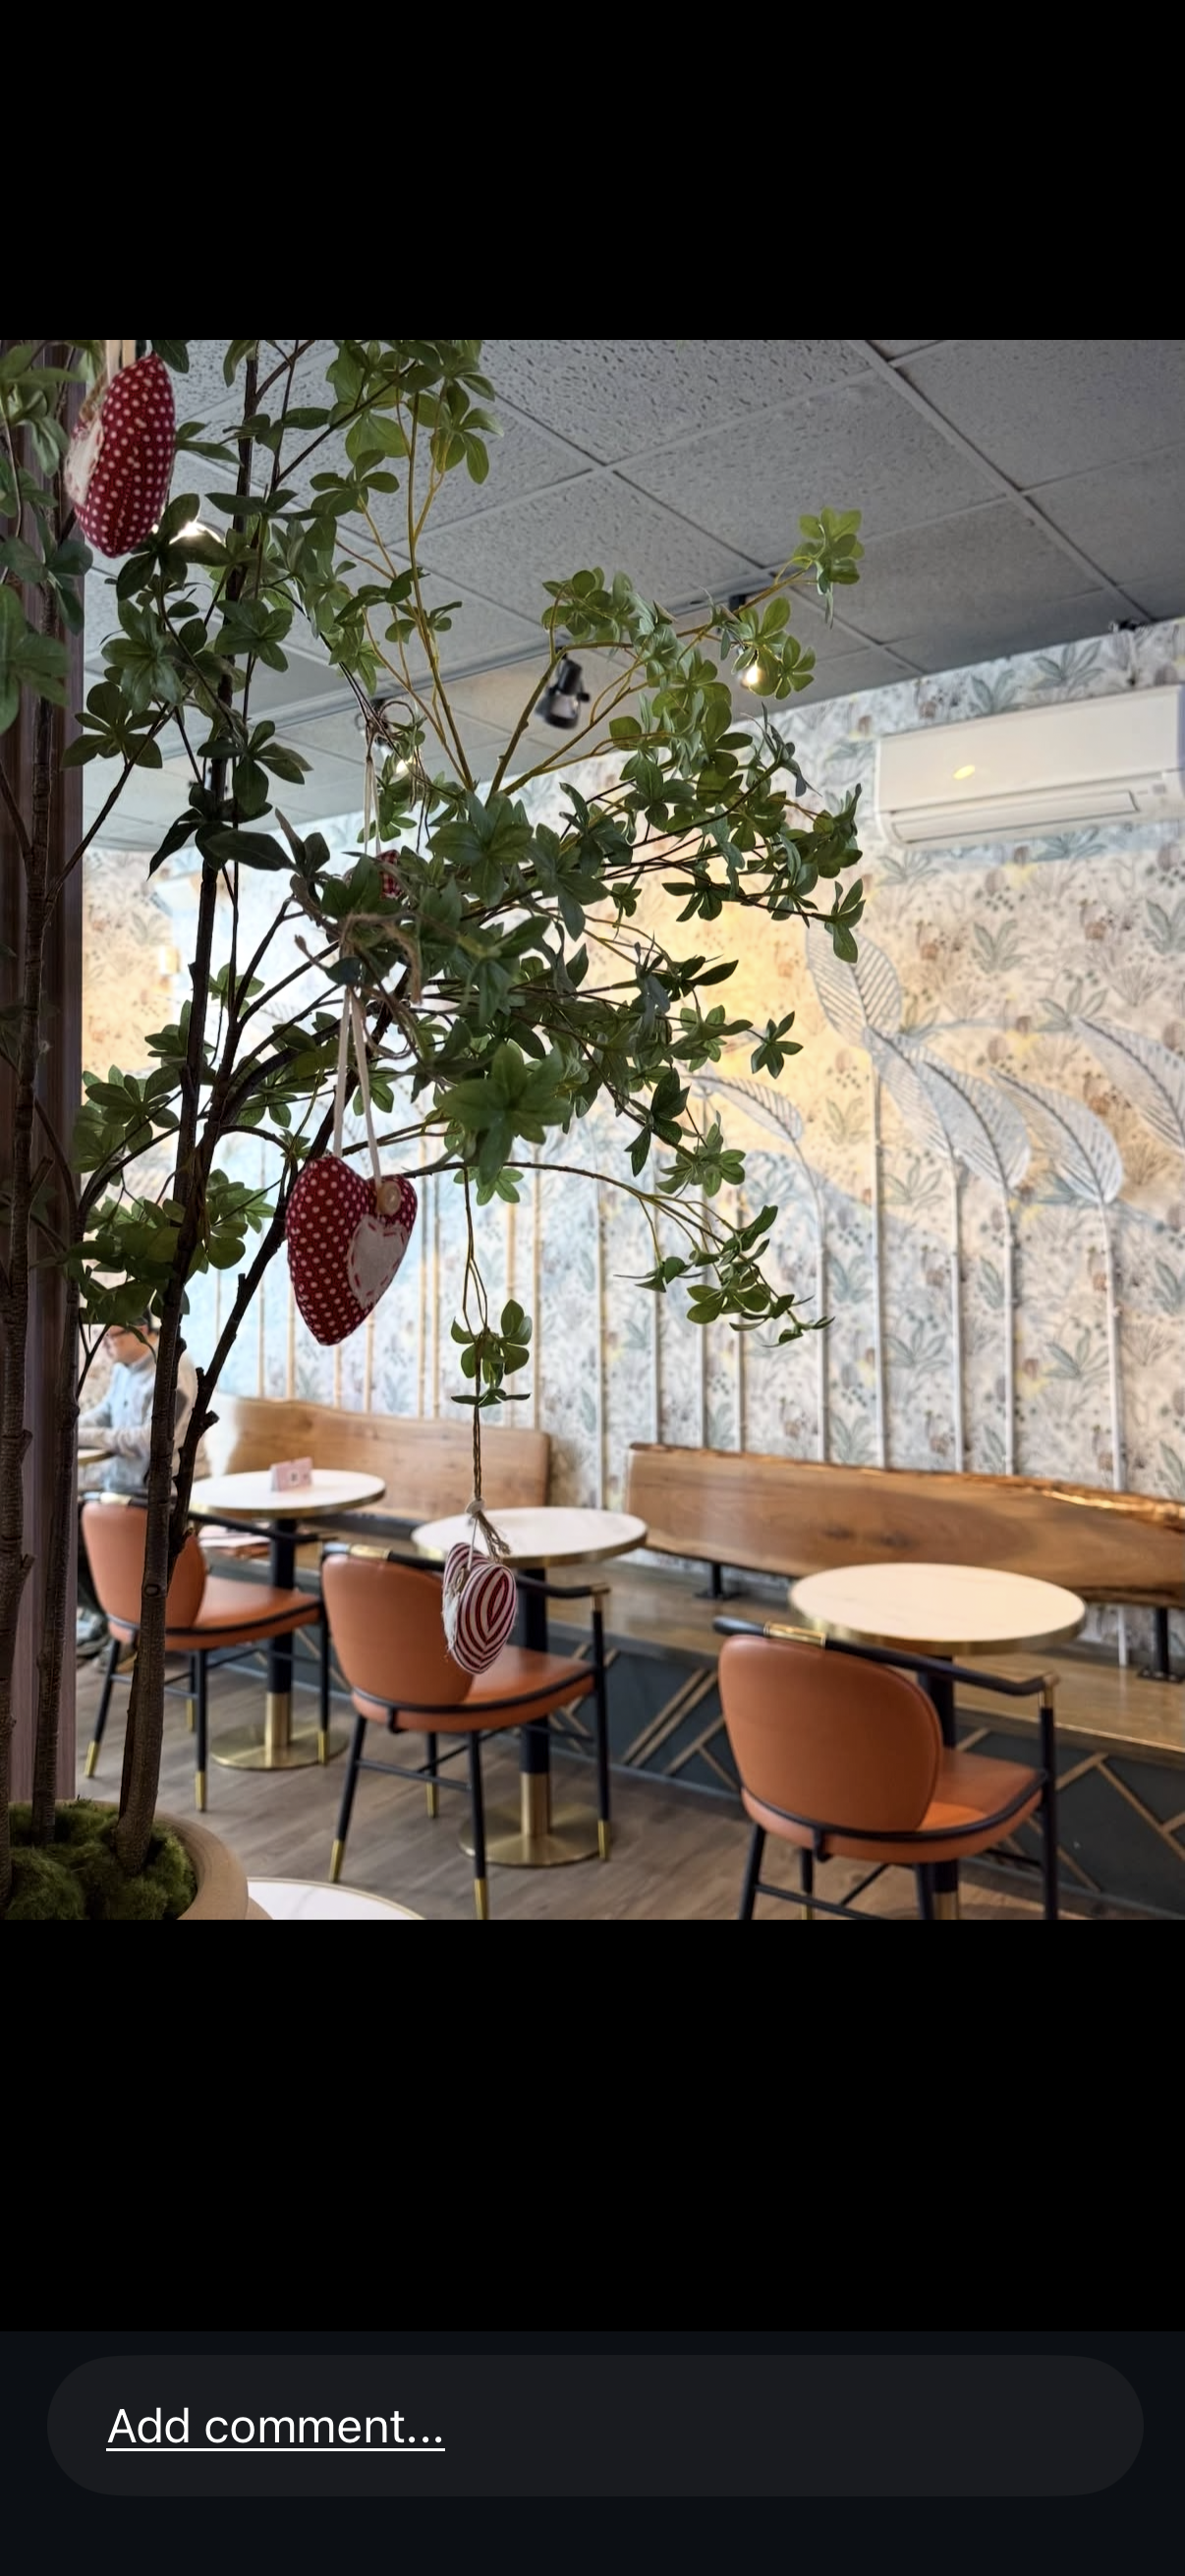
\includegraphics[width=\linewidth]{figures/ig_real_1.png}}
\end{subcaptionbox}
\hfill
\begin{subcaptionbox}{Real (street scene)\label{fig:igr2}}[0.40\linewidth]
{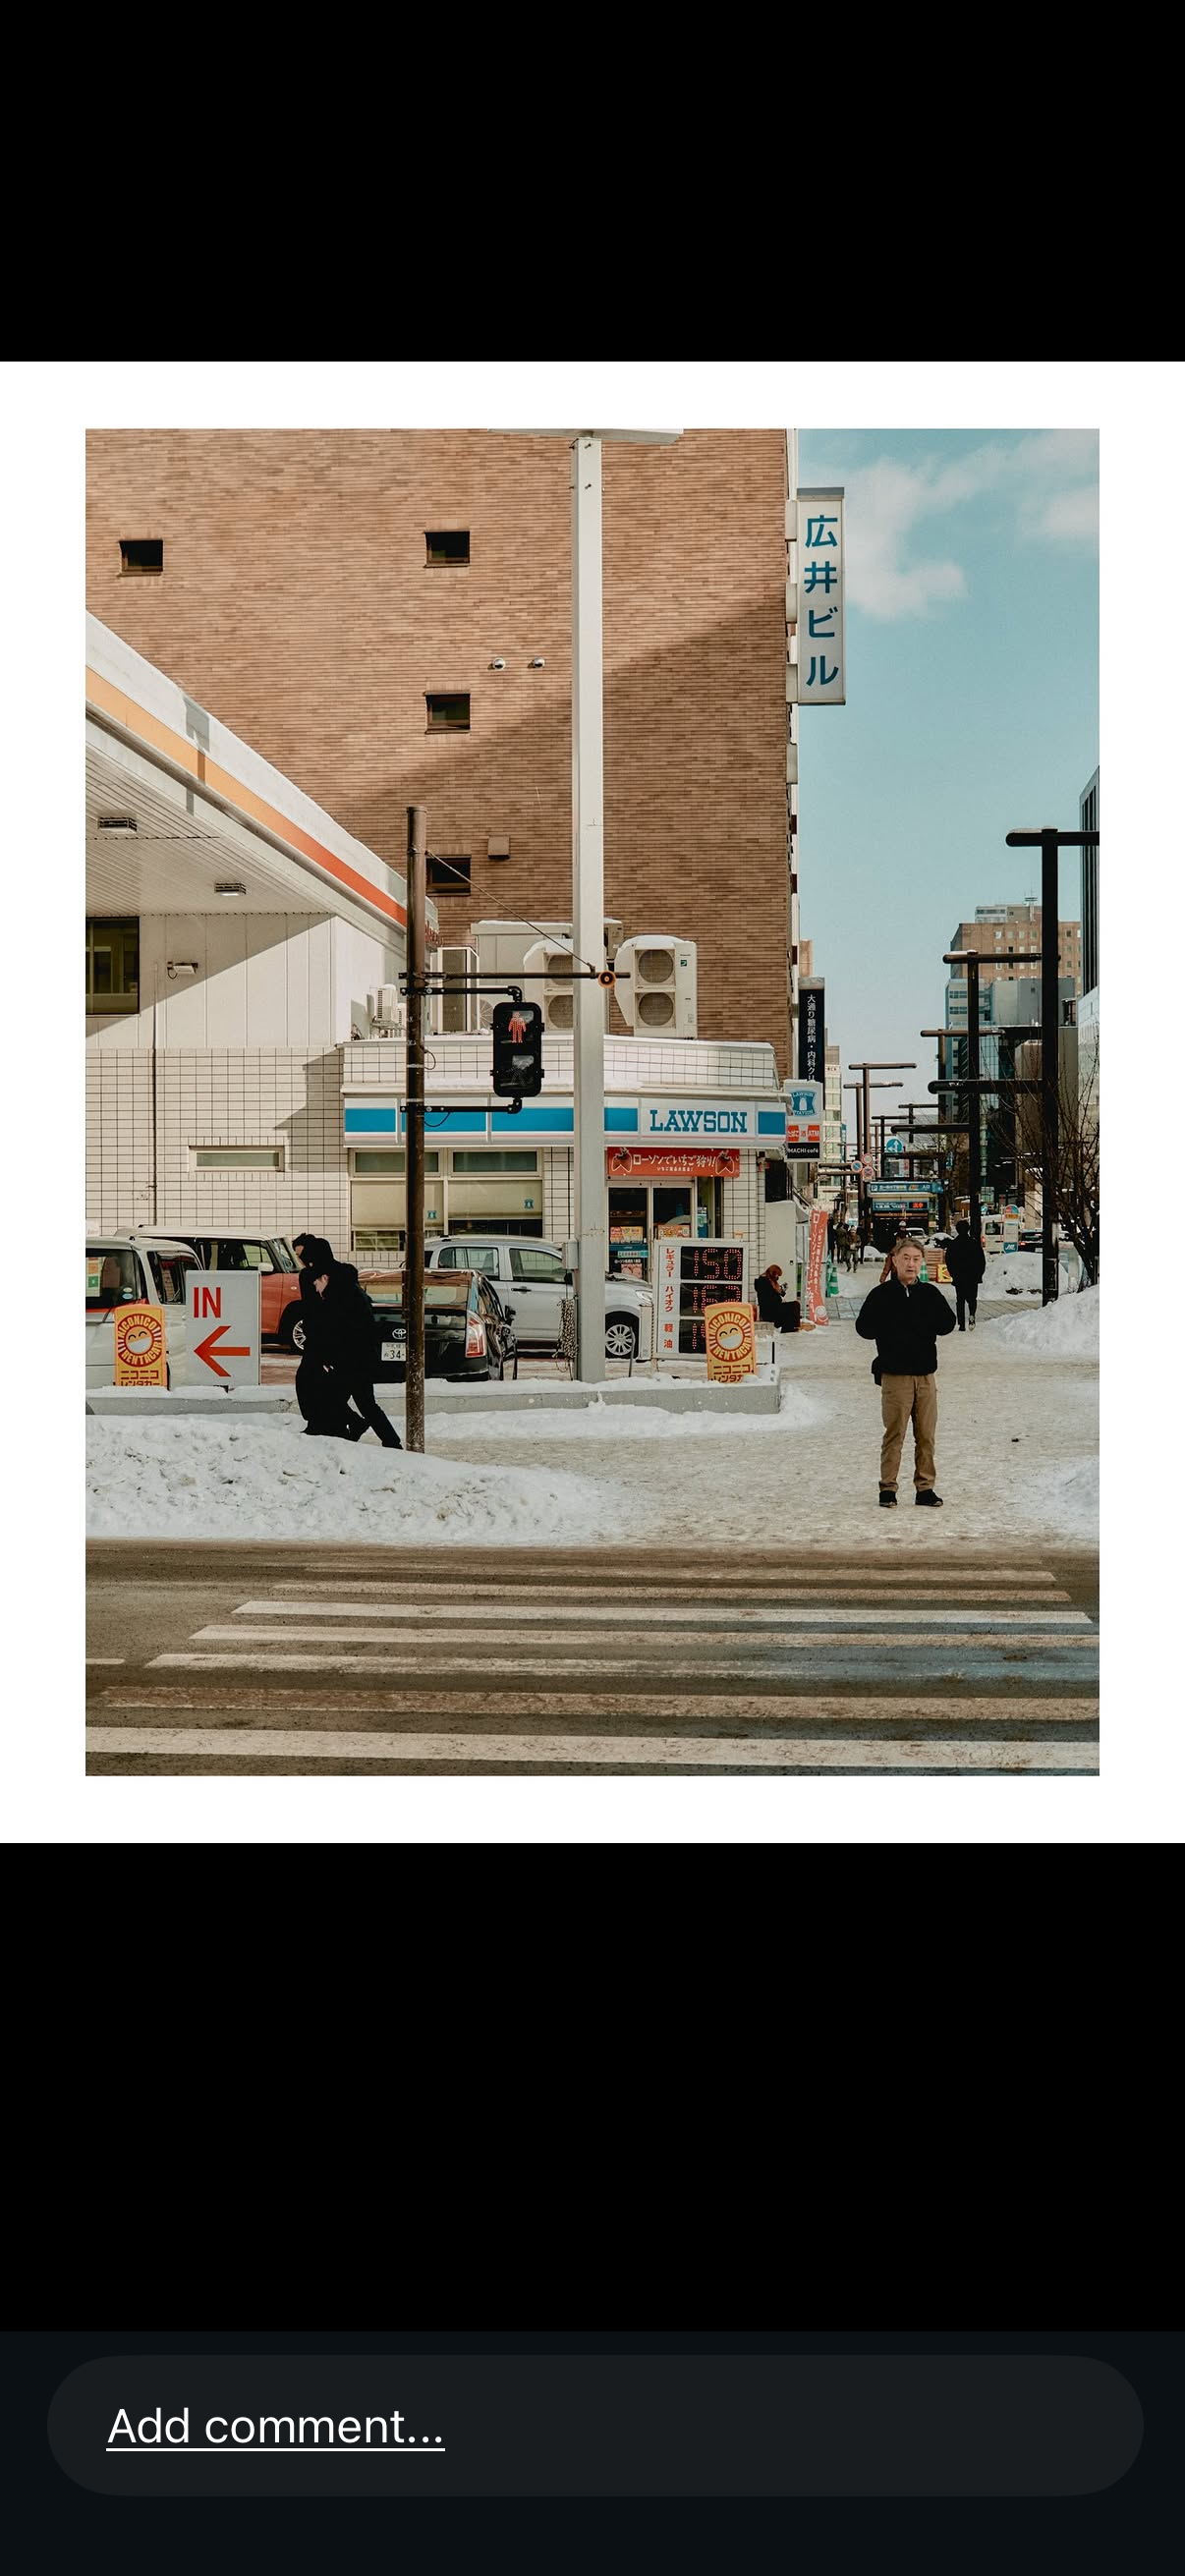
\includegraphics[width=\linewidth]{figures/ig_real_2.png}}
\end{subcaptionbox}
\caption{Four representative Instagram screenshots from my
manually collected evaluation set: (a)--(b) AI-generated, (c)--(d)
real human-photographed. Original content is the property of the
respective Instagram creators; included here for non-commercial
academic evaluation only.}
\label{fig:ig-grid}
\end{figure}

\paragraph{Gemini comparison.}
As an external sanity check, I uploaded a randomly drawn subset of
10 screenshots (5 real, 5 AI) to Google Gemini. In every response
it noted it could not detect any embedded watermark or SynthID
signature and therefore could not be 100\% sure. It returned brief,
hedged reasoning per image (lighting, skin texture, background
coherence) but did not commit to confident binary labels. This is
consistent with the expectation that screenshot recompression strips
cryptographic watermarks and that most third-party generators
(Midjourney, SDXL, Flux) never carried SynthID to begin with.

\subsection{Main results}
\label{sec:results}

Table~\ref{tab:main-results} reports clean and screenshotted
validation accuracies for all four ablation configurations and the
robustness gap $\Delta_{\text{gap}} = \text{ScreenshotAcc} -
\text{CleanAcc}$. The natural zero-effort baseline is the
\texttt{none} row (same backbone, no augmentation). Numbers come
from \texttt{runs/ablation/results.json}, produced by my Colab
notebook on 22~April 2026 (T4 GPU, 3 epochs, batch 64, AdamW
$\text{lr}=3\!\times\!10^{-4}$, cosine schedule, $10{,}000$ images
per class).

\begin{table}[t]
\centering
\begin{tabular}{lccc}
\toprule
Configuration                                                & Clean Acc.\ (\%) & Screenshot Acc.\ (\%) & $\Delta_{\text{gap}}$ (pp) \\
\midrule
EfficientNet-B0, \texttt{none}                               & 86.45            & 78.20                 & $-8.25$  \\
EfficientNet-B0, \texttt{screenshot}                         & 81.30            & 85.10                 & $+3.80$  \\
\textbf{EfficientNet-B0, \texttt{screenshot\_jitter}}        & \textbf{80.90}   & \textbf{86.45}        & $\mathbf{+5.55}$ \\
EfficientNet-B0, \texttt{screenshot\_jitter\_crop}           & 80.50            & 84.00                 & $+3.50$  \\
\bottomrule
\end{tabular}
\caption{Validation accuracy on the held-out clean and
\texttt{simulate\_screenshot}-perturbed CIFAKE splits. The bolded
\texttt{screenshot\_jitter} configuration is the deployed model. It
achieves the best screenshot accuracy and the most positive
$\Delta_{\text{gap}}$. Adding \texttt{RandomResizedCrop} on top
slightly hurts screenshot accuracy ($-2.45$~pp), suggesting crop and
screenshot augmentations partially compete in this regime.
Independent test-set evaluation on the 20{,}000-image held-out
CIFAKE test split confirmed the validation result: 79.49\% clean,
85.49\% screenshot, $\Delta_{\text{gap}}=+5.99$~pp.}
\label{tab:main-results}
\end{table}

\subsection{Calibration}
\label{sec:calib}
Before temperature scaling, the deployed
\texttt{screenshot\_jitter} model has an Expected Calibration Error
(ECE, 15~bins) of \textbf{10.0\%}. Fitting $T$ on the 2{,}000-image
validation set yields $T = 0.563$. Because $T < 1$, the rescaling
\emph{sharpens} the softmax outputs, indicating the raw model is
\emph{under}-confident, in contrast to the over-confidence typically
reported for modern deep networks~\citep{guo2017calibration}. I
attribute this to the heavy input-corrupting augmentations and the
short three-epoch schedule. After temperature scaling, ECE drops to
\textbf{1.9\%}: an 81\% reduction with one learned scalar.

\subsection{Real-world evaluation on Instagram}
\label{sec:realworld}

I run the deployed model ($T=0.563$) on the entire 49-image
Instagram set; per-class results are in Table~\ref{tab:realworld}.
This evaluation is intentionally distribution-shifted along three
axes: (a) content is not drawn from CIFAR-10 categories; (b) wild
AI generators are several generations newer (Midjourney~v6,
DALL\textperiodcentered E~3, SDXL, Flux) than CIFAKE's Stable
Diffusion v1.4; and (c) a real smartphone screenshot pipeline
includes status bars, UI chrome, and color profiles that
\texttt{simulate\_screenshot} does not model.

\begin{table}[t]
\centering
\begin{tabular}{lccc}
\toprule
Class           & $n$  & Accuracy / Recall (\%) & Mean confidence (\%) \\
\midrule
Real (human)    & 15   & 80.0                   & 89.4                 \\
AI-generated    & 34   & 14.7                   & 89.9                 \\
\midrule
\textbf{Overall}& \textbf{49}  & \textbf{34.7}  & \textbf{89.7}        \\
\bottomrule
\end{tabular}
\caption{Per-class accuracy and mean predicted confidence of the
deployed model on $n=49$ Instagram screenshots. Precision is 29.3\%
on real and 62.5\% on AI-generated.}
\label{tab:realworld}
\end{table}

The model achieves \textbf{34.7\% overall accuracy}: strong recall
on real photographs (80.0\%) and only 14.7\% on the AI class. It
confidently labels most modern AI Instagram content as ``real,'' and
mean confidence is $\approx 90\%$ on \emph{both} correct and
incorrect predictions, so the in-distribution calibration does not
transfer. I treat this as the headline finding of the real-world
evaluation: \emph{augmentation-aware fine-tuning closes the
synthetic robustness gap, but on its own it does not close the
real-world deployment gap.} A useful deployed detector requires
retraining on a contemporary mixed-generator corpus with screenshots
captured from real devices, not synthetically simulated. The full
report is at \texttt{runs/realworld\_report.json}.

% -------------------------------------------------------------
\section{Conclusion}
\label{sec:conclusion}

I presented a deliberately simple recipe for making an AI-image
detector robust to the most common real-world distribution shift,
the screenshot. Composing three physically motivated transforms
(JPEG recompression, down-then-up resampling, Gaussian blur) into
one \texttt{simulate\_screenshot} augmentation and wiring it into
the training pipeline of a frozen-backbone EfficientNet-B0 closes
the clean-to-screenshot robustness gap from $-8.25$pp on the
untrained baseline to $+5.55$pp on the deployed configuration,
without sacrificing clean-image accuracy. The system is deployed as
a calibrated, guardrail-gated Gradio application on Hugging Face
Spaces and reproduces in one Google Colab T4 session, satisfying
the Track~2 (Product Prototype) deliverable of ECE~57000.

\paragraph{Limitations.}
Training is dominated by CIFAKE's Stable-Diffusion-era outputs;
the Instagram evaluation confirms this generalization boundary. The
augmentation models compression, resampling, and softness, but not
cropping, overlays, or UI chrome. Heavily stylized real artwork can
also be misclassified as AI because the training distribution does
not separate ``non-natural appearance'' from ``synthetic origin.''

\paragraph{Future work and post-submission roadmap.}
Next steps are retraining on a contemporary mixed-generator corpus
(GenImage Flux/SDXL plus available Midjourney~v6) and expanding the
Instagram set from 49 to several hundred images. The GitHub
repository and Hugging Face Space are intentionally kept editable
so updated checkpoints and demo functionality can be pushed without
re-issuing the paper.

% -------------------------------------------------------------
\section*{LLM Acknowledgement}
\label{sec:llm}

Per the ECE~57000 rubric, large language model assistance is
disclosed here. The research question, problem framing, methodology,
\texttt{simulate\_screenshot} transform design, dataset choices,
ablation structure, manual collection and labeling of the Instagram
evaluation set, the Gemini comparison procedure, and the
interpretation of results are my own work, building on Checkpoint~1
(February~27, 2026) and Checkpoint~2 (March~29, 2026). Anthropic's
Claude was used as a writing and debugging assistant for prose
polishing, LaTeX formatting, code scaffolding around the verbatim
snippets I authored, and Python error resolution during Colab
execution. The LLM did not generate experimental results, design
the methodology, or access any course systems. A companion
\texttt{LLM\_ACKNOWLEDGEMENT.md} in the repository mirrors this
disclosure.

% -------------------------------------------------------------
\bibliographystyle{iclr2026_conference}
\bibliography{references}

\end{document}
